\documentclass[10pt,conference]{IEEEtran}


\title{\LARGE \bf Automatic Estimation of FM Synthesis Parameters by Convolutional Neural Network}

%\usepackage{hyperref}

% \hypersetup{allcolors=black,
%             linkbordercolor={1 1 1},
%             urlbordercolor={1 1 1}}


\usepackage{multirow}
\usepackage{subfig}
\usepackage{balance}
\usepackage{booktabs}
\usepackage{graphicx}
\usepackage{color}
\usepackage{multirow}
\usepackage{subfig}
\usepackage{balance}

\newcommand{\basg}[1]{{\color{blue}[#1]}}
\newcommand{\sergio}[1]{{\color{red}[#1]}}


\begin{document}

\author{Anonymous Authors}

\maketitle
\thispagestyle{empty}
\pagestyle{empty}

\begin{abstract}
FM synthesis is one of the most renowned techniques for sound synthesis, and although it is an old method, it remains widely used today. It is simple, computationally inexpensive, and capable of producing high-quality results. However, the successful use of this type of audio synthesis presents a significant challenge: selecting the correct synthesizer parameters. This process is not precise, and there is no fully deterministic procedure to follow. Musicians are usually guided by intuition and an empirical trial-and-error process. To revive this technique and leverage its benefits, using CNN models appears to be a very promising option, as they can help musicians achieve convincing results, imitate real instruments quickly and at low cost, and even create entirely unpredictable timbres and effects. Therefore, this work explores this approach by creating a pipeline capable not only of training a CNN model to predict the appropriate parameters that enable an FM synthesizer to resynthesize original audio samples (such as acoustic instruments), but also of exploring the synthesizer’s parameter space broadly, allowing it to reproduce any arbitrary desired sound. The proposed approach proved to be efficient for both objectives: the developed model was able to approximate unseen sound samples (of real instruments), and the error metrics converged to satisfactory values even when using an exploratory dataset generation process (a synthetic dataset specifically constructed to explore the FM synthesizer’s capabilities).
\end{abstract}

\begin{IEEEkeywords}
Music, FM synthesis, CNNs
\end{IEEEkeywords}


\section{Introduction}

Musical expression is one of humanity’s earliest experiences and one of the most valued forms of art. This art form has been cultivated since ancient times. The Chinese, three thousand years before Christ, had already developed complex systems of musical theory, and Greek culture not only cultivated the study of music but also associated it with religion, assigning divine characteristics to protect and honor music itself~\cite{med1996teoria}.

Although music is a subjective form of human knowledge, the recorded music industry generates approximately US\$29 billion annually~\cite{ifpi2025}, so its value is no longer purely subjective. It is precisely in this context that the artifice of synthesized sound appears in history. It emerged after the first electronic instruments and, due to the periodic nature of sound, the earliest synthesizers were composed of simple analog oscillators that could be manually controlled through operations such as summing and filtering~\cite{holmes2016electronic}.

In the 1980s, with the release of the Yamaha DX7 synthesizer, the history of music synthesis took a major turn. The Yamaha DX7 marked the first major success of a revolutionary technique developed by John M. Chowning at Stanford University and later popularized by Yamaha~\cite{claesson2021resynthesis}. This event marked a new milestone in sound synthesis, not only because of its popularity but also because it made reproducing both realistic instrument simulations and entirely new sounds easily accessible to musicians and composers of all levels. In fact, the success of FM synthesis was so great that the technique remains in use to this day~\cite{holmes2016electronic}.

Thus, the primary goal of the present work is to guide a frequency-modulation (FM) synthesizer to reproduce instrument sound samples, while also developing a process that fully explores the expressive capabilities of the FM synthesizer itself, thereby approximating the re-synthesis of any input sound. This approach aligns with one of the key historical advantages of FM synthesizers: their ability to create sounds that cannot be produced by traditional acoustic instruments.

Although FM synthesis is considered an old technique compared to newer approaches such as wavetable synthesis or GAN-based sound generation, it remains widely used within today’s complex musical ecosystem due to its advantages: it is easy to use, well-suited for experimenting with new and even unpredictable sounds (such as spatial effects), and easily adaptable to real-time composition. So, researchers continue to focus on improving the control of traditional FM synthesis parameters (which, when done manually, can be a tedious empirical process). For instance, \cite{claesson2021resynthesis} implemented a neural network to predict FM synthesizer parameters from frequency-domain sound representations. Similarly, \cite{steinmetz2022ddx7} proposed an interesting TCN-based approach that couples the FM synthesizer directly into the network training process.

The current work, however, wants to employ a Convolutional Neural Network (CNN)~\cite{LeCun1989}~\cite{alexnet} to achieve its goals, because CNNs enable the direct use of raw audio samples as model input while serving as an excellent feature extractor for sound signals~\cite{kiranyaz2021survey}. CNNs are also well known for their ability to economize computational resources when handling high-dimensional data. Therefore, CNNs are a strong candidate for this type of research task.

Furthermore, beyond a simple resynthesis exercise, the present work aims to develop a process that enables the model to achieve a broad understanding of the parameter space of the applied FM synthesiser. The idea behind the proposed methodology is that if the model can learn the FM synthesizer’s parameter space in a comprehensive way, it can then be used to simulate any sound within the synthesizer’s capabilities, making the experience of a hypothetical future user (a musician or composer) much more efficient in achieving any desired sound (allowing good integration into real compositions workflows).

The remainder of this paper is organized as follows. Section~\ref{sec:fund} presents the fundamental concepts related to music. Section~\ref{sec:related} discusses the related work. Section~\ref{sec:our_proposal} describes the details of the proposed approach and the experimental setup. Section~\ref{sec:experiments} presents and analyzes the results. Finally, Section~\ref{sec:conclusion} provides the conclusions of this work and outlines directions for future research.

\section{Musical concepts} \label{sec:fund}

Musical computation is a broad, interdisciplinary field that encompasses the computational processing of music and sound. A comprehensive overview is beyond the scope of this paper; however, for the present study, a basic understanding of key sound properties is necessary, particularly in the context of synthesis and re-synthesis tasks:

\textbf{Timbre} is commonly described as the ``color'' of sound. From a signal-processing perspective, it is determined by the distribution, relative amplitudes, and temporal evolution of the harmonic components present in an audio signal. In acoustic instruments, these components arise from multiple simultaneous vibration modes, whose behavior depends on physical characteristics such as material, geometry, and excitation mechanism. This complex interaction produces a distinctive spectral structure that characterizes each instrument’s timbre. To analyze this property, audio signals are commonly transformed from the time domain to the frequency domain using Fourier-based techniques~\cite{benson2008music}.

\subsection{Audio digitization}

To digitize an audio signal, a process known as sampling is used~\cite{po2022sampling}. For human hearing, a sampling frequency of 20~kHz is generally sufficient. However, when focusing on musical instruments, a sampling rate of 16~kHz is often adequate. Therefore, to ensure compatibility with the NSynth dataset (presented below), this work uses an audio sampling rate of 16 kHz.

\subsection{Frequency Modulation Sound Synthesis}

One of the most popular sound synthesis techniques is Frequency Modulation Synthesis (FM Synthesis), introduced by John M. Chowning~\cite{chowning1973synthesis}, who explored the effects of frequency modulation at high frequencies near the audible range, rather than the traditional use of inaudible frequencies. In summary, the FM synthesis technique allows the addition of multiple sidebands around the base frequency for each modulator used in the synthesizer algorithm. As a result, rich spectral audio can be created using only a few modulators, and a sound designer can, through an empirical process, create arbitrary sounds by adjusting the synthesizer parameters~\cite{lazzarini2023higherorder}.

This type of synthesis was popularized by the Yamaha DX7 synthesizer and remains in use today due to its efficiency, low computational cost, and flexibility~\cite{steinmetz2022ddx7}.

\subsection{Audio comparison}

The task of audio comparison is not straightforward, especially when the goal is to achieve perceptual similarity from a human hearing perspective. It can be complex, computationally demanding, and inherently subjective; however, several well-established and efficient methods can address this challenge.

According to~\cite{claesson2021resynthesis}, three metrics are commonly used for this purpose. The \textbf{FFT distance} is computed by applying the Fast Fourier Transform (FFT) to the two audio samples and measuring the Euclidean distance between their spectra, typically normalized to the $[0,1]$ range. The \textbf{Short-Time Fourier Transform (STFT) distance} follows the same principle but is calculated over short, overlapping time windows, providing time-localized spectral information. Finally, the \textbf{Log-Mel spectrogram distance} is based on the Log-Mel representation, which adapts the FFT spectrum to better reflect human auditory perception by mapping linear frequencies onto the Mel scale~\cite{claesson2021resynthesis,chulev2024improving}.

In addition to these metrics,~\cite{claesson2021resynthesis} also recommends the use of the Euclidean distance between amplitude envelopes. While this approach is valuable for evaluating temporal dynamics, the present work focuses specifically on timbral similarity; therefore, envelope-based comparisons are outside the scope of this study.

\section{Related Work} \label{sec:related}

Several studies have explored the use of machine learning to estimate parameters for sound synthesizers. The main contribution of the present work lies in the use of convolutional neural networks (CNNs) operating directly on raw audio signals. CNNs are particularly well-suited for this task because they can process high-dimensional inputs, capture temporal structures in audio signals, and provide near-real-time inference after training.

\cite{claesson2021resynthesis} proposed the re-synthesis of instrumental sounds using machine learning models combined with an FM synthesizer. In that work, however, CNNs and raw audio were not used; instead, the input consisted of STFT spectrograms, a frequency-domain representation that may simplify learning but does not fully exploit temporal information present in the signal.

\cite{steinmetz2022ddx7} introduced DDX7, a differentiable FM synthesizer designed for the re-synthesis of musical instrument sounds. Their approach employs a Temporal Convolutional Network (TCN) and integrates the Mel-spectrum directly into the loss function, aligning optimization with perceptually motivated audio metrics. While effective, this method requires embedding the synthesizer in the training loop, which increases computational and memory costs. In contrast, the present work emphasizes generalization through large-scale randomized exploration of the FM parameter space, without incorporating the synthesizer into the optimization process.

Finally, \cite{kiranyaz2021survey} presented a comprehensive survey of one-dimensional CNNs and their applications, highlighting their effectiveness for sequential data such as audio signals. This work supports the suitability of CNN-based architectures for learning temporal patterns directly from raw audio.

\section{Methodology} \label{sec:our_proposal}

This section introduces our proposed approach of using AI to guide an FM synthesizer in simulating any instrument or any desired sound. More specifically, we propose a Convolutional Neural Network (CNN) to analyze a sound signal sample and predict the correct parameters of an FM synthesizer to re-synthesize the ``same'' timbre, enabling the synthesizer to simulate the desired ``voice'' playing any song. Since this idea is still quite abstract and broad, we consider the following steps:

\begin{enumerate}
    \item \textbf{Implementing FM synthesizer:} Implement a simple FM synthesizer, which can later be used both to generate the dataset and to test the ability to re-synthesize a sound.
    \item \textbf{Generating the dataset:} Generate a synthetic audio dataset composed of random samples, each created by randomly selecting FM synthesizer parameters. This essentially records tuples of [audio sample; parameter values] (where the parameters are the target values) and explores the parameter space at a large scale.
    \item \textbf{Training the CNN:} Train a CNN to predict the correct parameters for the same FM synthesizer, given only an audio sample.
    \item \textbf{Evaluating the Model:} Evaluate the model's results using the NSynth dataset to test its generalization capabilities.
\end{enumerate}

Frequency Modulation Synthesis was chosen because it is one of the most common and effective methods for generating audio samples, owing to its simplicity and low computational cost. However, the effective use of this technique requires advanced knowledge to select the correct parameters to achieve good results.

% This technique became extremely popular in the 1980s with the release of the Yamaha DX7 synthesizer. By the 1990s, it had become a standard for many commercial synthesizers and remains in use today in electronic music production (\cite{claesson2021resynthesis}). However, the effective use of this technique depends on advanced knowledge to select the correct parameters for generating good results, which can involve thousands of parameters.

Therefore, the ability to simplify parameter selection provides strong justification for this study, and AI models appear to be an affordable way to learn the right patterns for controlling an FM synthesizer. The basic idea is that a model can be trained to guide an FM synthesizer in mimicking any sound, thereby reducing the effort required to compose electronic music.

Furthermore, in terms of computational cost, using an AI model to predict parameters and guide an FM synthesizer is much more effective than applying a Generative Neural Network to generate an audio. Additionally, a synthesizer is particularly well-suited to real-time composition and electronic music performance.

Regarding the configuration aspects, all experiments were conducted in an environment composed of Python (3.11.2), TensorFlow (2.19.0), Keras (3.11.1), Nvidia CUDA (12.5.82), Nvidia cuDNN (3.0.75), Nvidia driver (535.247.01), and CUDA (12.2), using an NVIDIA GeForce GTX 1650 GPU with 4GB of memory.

\begin{figure}[htd]
    \centering
    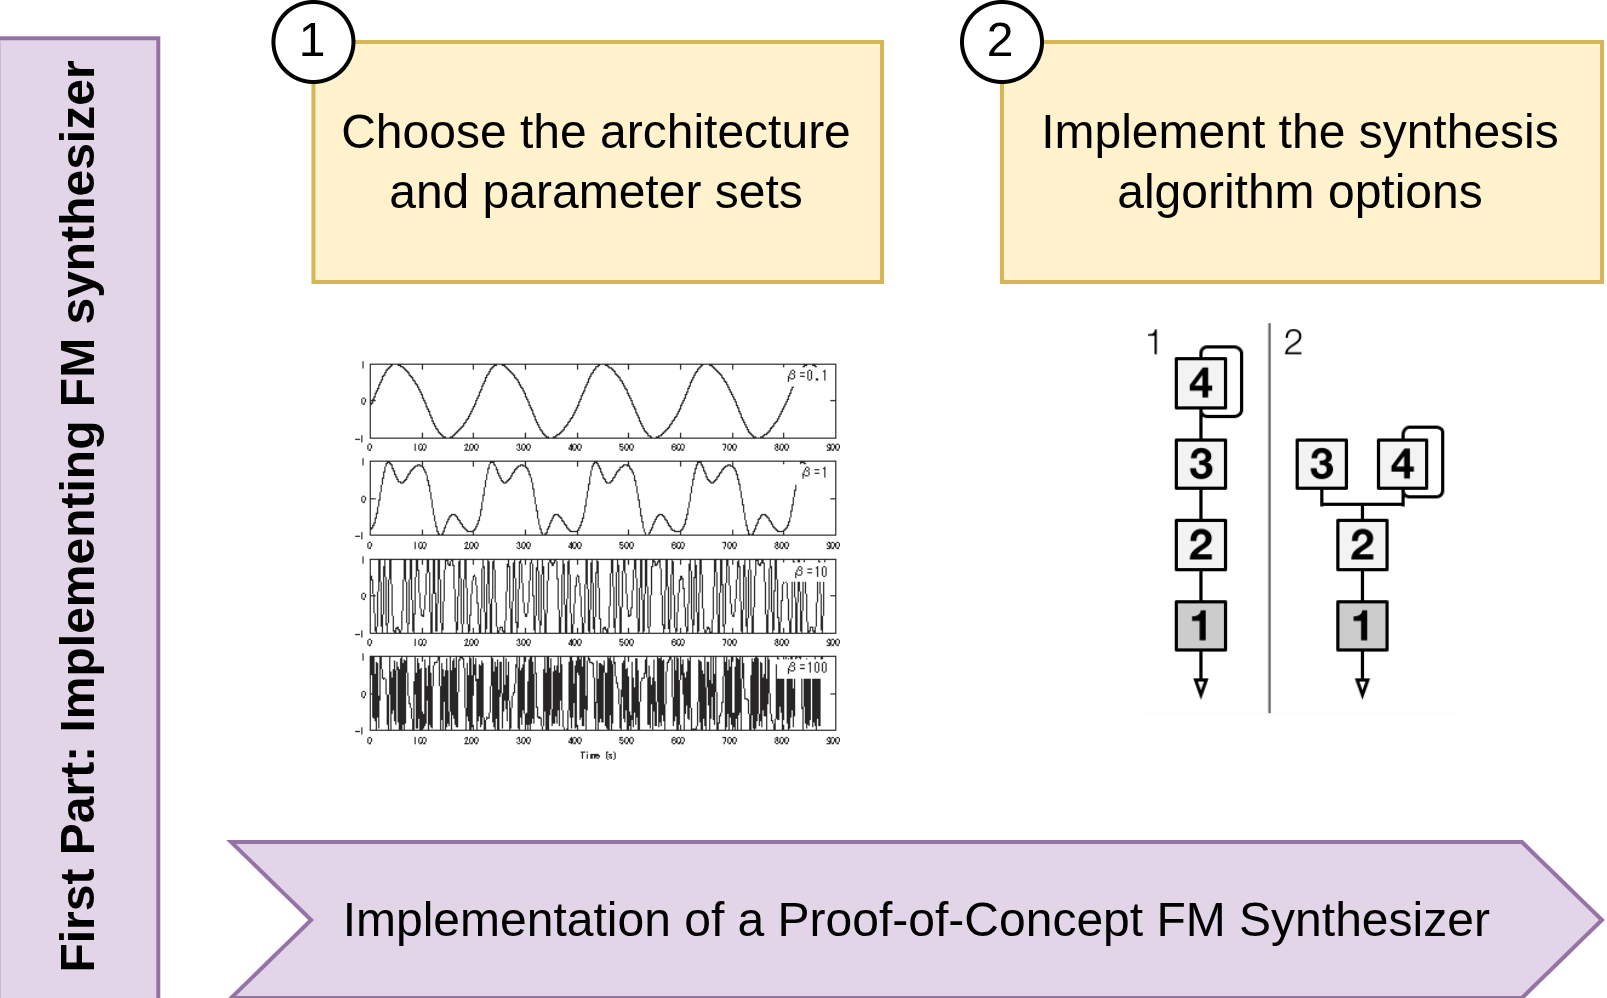
\includegraphics[width=1\columnwidth]{figs/first_part.png}
    \caption{Synthesis implementation and dataset generation.}
    \label{fig:met1}
\end{figure}

\subsection{Implementing FM synthesizer}

There are several well-known FM synthesizers on the market, but most are not open-source. Additionally, commercial synthesizers often have numerous parameters to control the audio production process. For example, Native Instruments' FM8 can use around 1,000 parameters~\cite{claesson2021resynthesis}, and Teenage Engineering’s OP-1 synthesizer can be configured with up to $10^{76}$ parameters~\cite{claesson2021resynthesis}.

This large number of parameters is intended to give users fine-grained control over the generated audio, allowing for a wide variety of pitches (simulating a broad range of instruments and even non-instrument sounds, such as bird songs or car horns). However, since this project is focused on research rather than a commercial solution, a simple FM synthesizer will suffice.

The implemented FM synthesizer has only 6 operators, inspired by the classic Yamaha DX7, which was one of the most disruptive milestones in the history of electronic music composition. In fact, this simple setup is enough to cover all FM synthesis theories and achieve good performance during AI model evaluation. In summary, the implemented FM Synthesizer (Figure~\ref{fig:FMSynth}) consists of 5 modulator operators, 1 carrier operator, 1 ADSR envelope, and 2 synthesis algorithms (one completely serial, and another with 3 serial operators followed by 2 parallel operators).

\begin{figure}[h] 
    \centering
    \includegraphics[width=.9\linewidth]{figs/algs2.png}
    \caption{FM Synthesizer Algorithms.}
    \label{fig:FMSynth}
\end{figure}

To summarize, the implemented synthesizer renders the audio signal according to the following steps:

\begin{enumerate}
    \item Generate each operator signal by applying it to modulate the phase of the next operator in the sequence. In this implementation, only the phase is varied (similar to the Yamaha DX7), whereas a full FM synthesis would also be able to vary the frequency. This simplification helps to avoid complex noise-handling issues and promotes numerical stability. All signals are rendered at a 48 kHz sample rate.
    \item Combine the output of each operator according to the synthesis algorithm (when there are parallel operators, they are summed).
    \item Apply the ADSR envelope to the signal.
    \item Downsample the signal from 48 kHz to 16 kHz (applying also a low-pass filter to avoid aliasing).
\end{enumerate}

It is important to highlight that the high sample rate of 48 kHz was chosen to allow the FM synthesis to work well enough, since at high frequencies, there is a risk of obtaining aliasing and noise (due to the extremely high frequency components generated by the normal spacing of the FM operators). Furthermore, the low-pass filtering, used to downsample, is also useful to prevent the aliasing problem (after the downsampling process).

Finally, it is important to highlight that the entire synthesizer relies on 16 input parameters, consisting of the beta and ratio values for each modulator and for the carrier (totaling 12 parameters), plus 4 parameters for the ADSR envelope (attack, decay, sustain, and release times). As mentioned earlier, it is a very simple FM synthesizer, yet fully featured and sufficient for the purposes of the current research.

\subsection{Generating the dataset}

\begin{figure}[h]
    \centering
    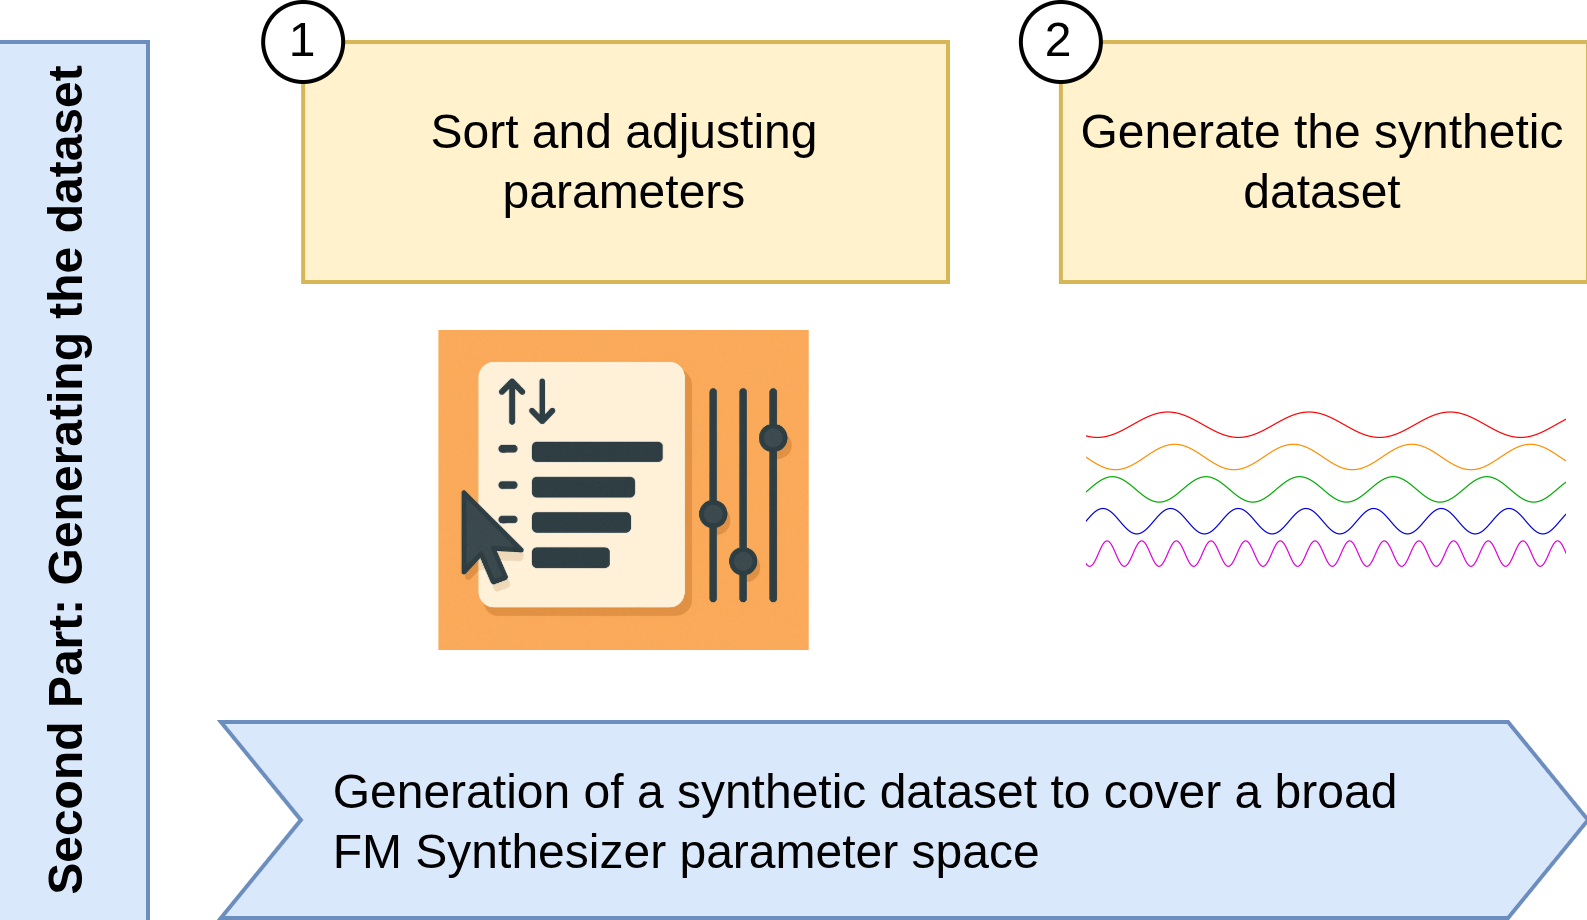
\includegraphics[width=1\columnwidth]{figs/second_part.png}
    \caption{Synthesis implementation and dataset generation.}
    \label{fig:met1}
\end{figure}

This work utilizes two datasets, each serving a distinct purpose: the generated dataset, referred to below as the synthetic dataset, which is used for training; and the NSynth dataset, which is used to evaluate the model’s generalization capabilities. However, in this section, only the first dataset will be considered, while the second will be addressed in Section~\ref{sec:evaluation_method}.

One of the most challenging steps in the KDD process is obtaining and processing data. However, for the purposes of this work, an effective approach can be used. Similar to Claesson's approach~\cite{claesson2021resynthesis}, since the goal is to achieve good control over the synthesizer parameters, it is sufficient to generate many samples of synthesizer parameters and their respective audio outputs.

The dataset used to train the model will consist of 5{,}000 samples generated by the implemented FM synthesizer, each with a duration of 4 seconds, monophonic audio (single-channel), a 16 kHz sample rate (with samples originally generated at 48 kHz and subsequently downsampled to ensure compatibility with the NSynth dataset), pitches varying between 20 Hz and 6{,}000 Hz, and randomly generated ADSR envelopes.

The expectation is to achieve a level of learning where the model can accurately predict the parameters for a wide range of sounds that can be generated by the implemented FM synthesizer.

However, as the main purpose is to re-synthesize real instrument samples, the randomness of this dataset should be controlled to achieve reasonable music property samples, or, in other words, the dataset was constructed respecting the well-known limits and characteristics of real instruments:

\begin{itemize}
    \item The minimum frequency for the carrier is 20 Hz, and the maximum is 6 kHz (for example, the maximum frequency for a violin is approximately 3 kHz; another important aspect for this maximum choice is that we need to stay under 8 kHz due to the output sample rate, because of the Nyquist frequency). The frequency is chosen by a uniform random distribution.
    \item The minimum ratio for each modulator is 1/8, and the maximum is 8 (to avoid aliasing in the final signal). Two methods are used to select the ratio: a) with 90\% probability, the ratio will be a random uniform choice between discretized values (for example: 1/8, 1/6, ..., 2, 3, 54, ..., 8; the idea is to simulate a real instrument); and b) with 10\% probability, the ratio will be a uniform log distribution between 1/8 and 8 (allowing random metallic sounds, like bells, but respecting human auditory perception, where the difference between low frequencies is more perceived than between high frequencies).
    \item The minimum beta is 0, and the maximum is 8 (also to avoid aliasing in the final signal). The beta is chosen by a uniform random distribution, controlled such that 20\% of the values are between 0 and 0.5, 60\% are between 0.5 and 3, and 20\% are between 3 and 8 (prioritizing rich timbres and avoiding pure sinusoidal sounds, as well as excessive metallic sounds).
    \item The amplitude is fixed at 1.0, to avoid different combinations of beta and amplitude generating the same frequency spectrum and the same timbre (prioritizing the CNN learning).
\end{itemize}

Regarding the ADSR envelope, the attack, decay, sustain, and release parameters were randomly sampled from uniform distributions within predefined intervals. Specifically, the attack time ranged from 0.005 to 0.5~s, the decay time from 0.02 to 0.6~s, the sustain level from 0.1 to 0.9, and the release time from 0.05 to 0.8~s.

With these additional adjustments, the synthetic dataset will be more representative of simulating real instruments.

As each sample in the generated dataset is a complete 4-second sound (containing 64,000 audio samples, which corresponds to 16 kHz multiplied by 4 seconds), so a simple 75/25 train-test split was used, resulting in 3,750 audio files for training and 1,250 for testing.

But, from these 3,750 audio files, 20\% of them will be used for validation, resulting in a total of 3,000 samples for training and 750 samples for testing.

\subsection{Training the CNN}

As described in Section~\ref{sec:fund}, the main characteristic of the sound that should be reproduced to achieve the main work goal is the ``timbre``, which is defined as the combination of frequencies present in the sound. It is clear that techniques such as filtering and Fourier Transform can be used to extract timbre components from an audio signal; however, they are insufficient for controlling an FM Synthesizer. In fact, the FM Synthesis control is, normally, an experimental process involving trial and error.

Additionally, each FM Synthesis operator generates additional frequency components in the signal, and there is no practical method to predict the correct parameter settings. However, as a mathematical function, it is easy to see that this synthesis pattern can be easily approximated using AI models.

Thus, the current work aims to use a CNN model, since it is a very effective method for learning patterns, respecting the internal data structure, and without requiring extensive preprocessing work. In other words, a CNN can simultaneously learn the time-dependent aspects of an audio signal and can act as a pattern extractor by applying a sequence of filtering operations, allowing the use of the raw audio format as input.

To train the CNN model, the already presented synthetic dataset will be used. Its main advantage is that it contains both the audio signal and the corresponding parameters used to generate each sample. In addition, this approach covers a wide range of the parameter space.

Consequently, the training process is straightforward and is expected to yield good performance.

Figure~\ref{fig:met2} presents the overall scheme of this training process.

\begin{figure}[h]
    \centering
    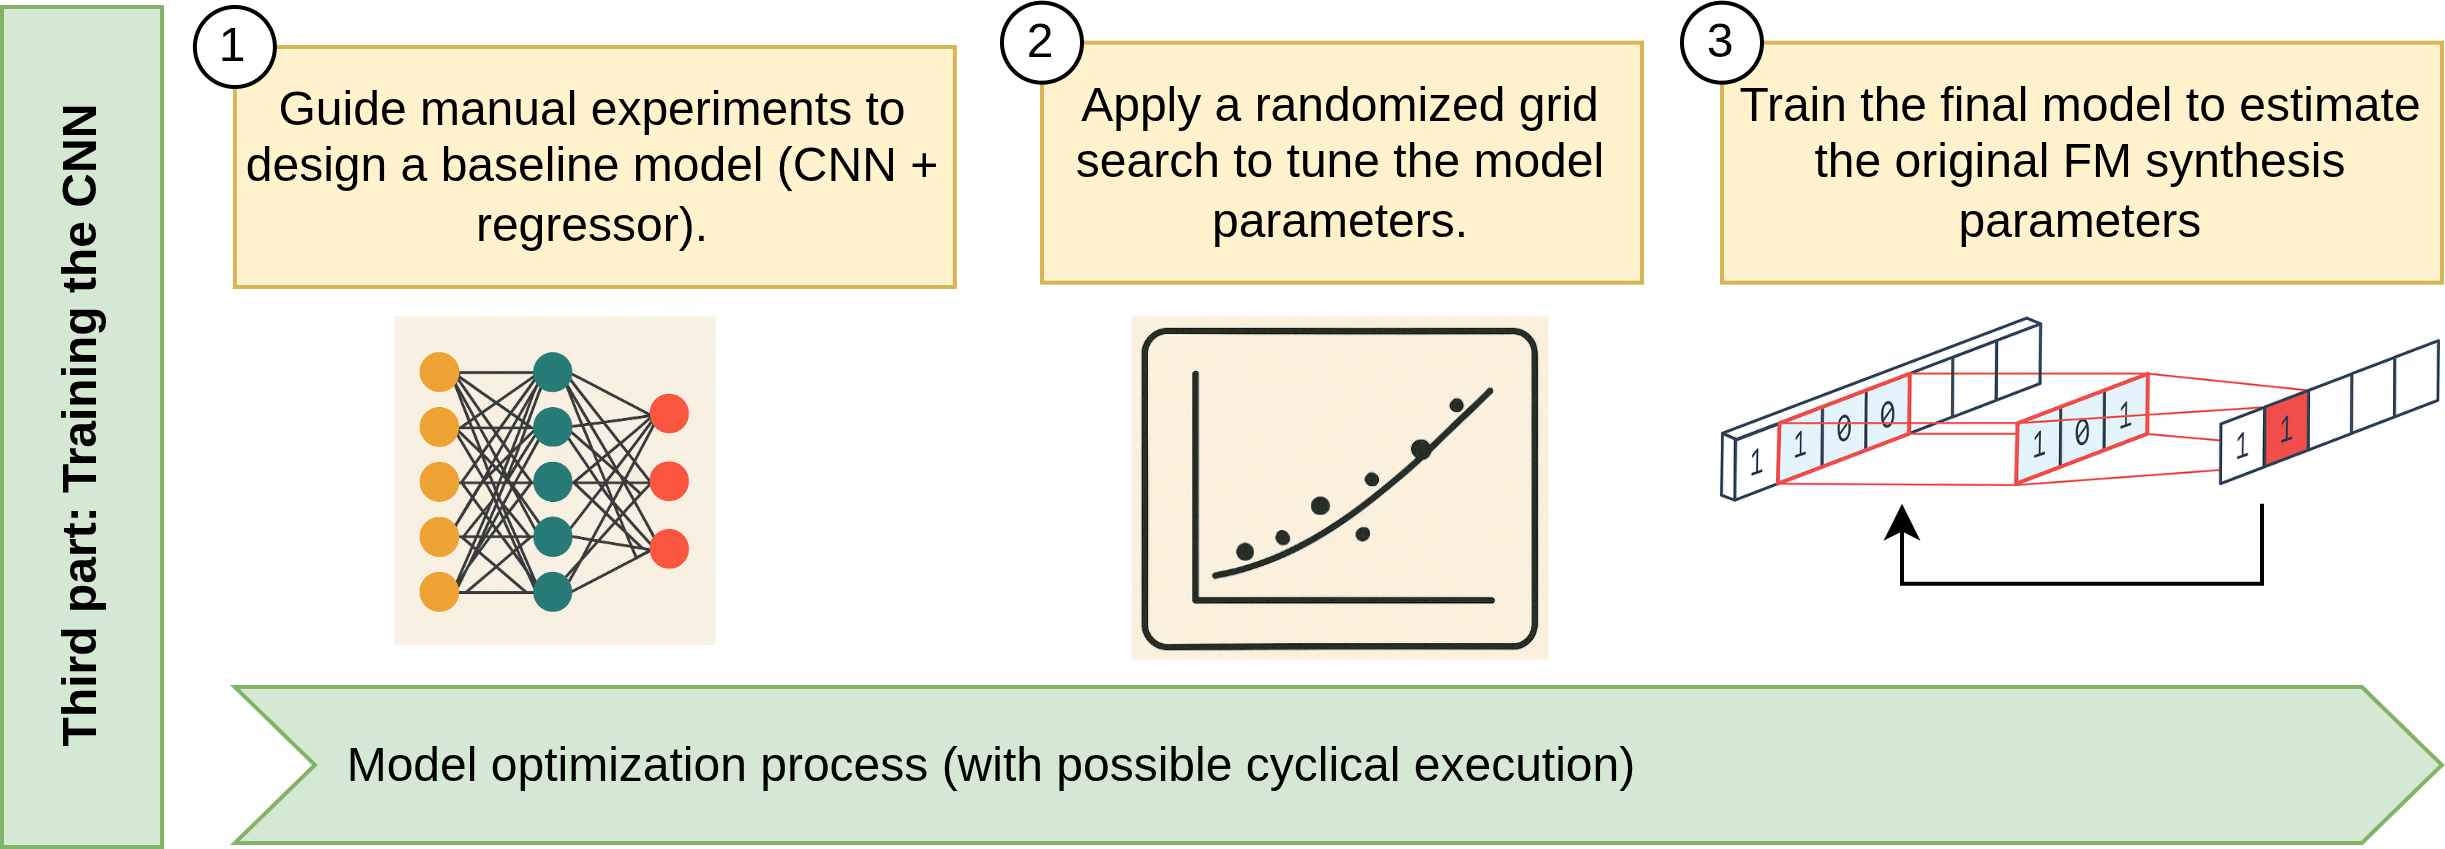
\includegraphics[width=1\columnwidth]{figs/thrid_part.png}
    \caption{Model training and optimization.}
    \label{fig:met2}
\end{figure}

The model architecture used is as follows, where the first covers the feature extraction (CNN), and the second covers the regression (a common MLP):

\begin{figure}[h]
    \centering
    \subfloat[][Feature extration]{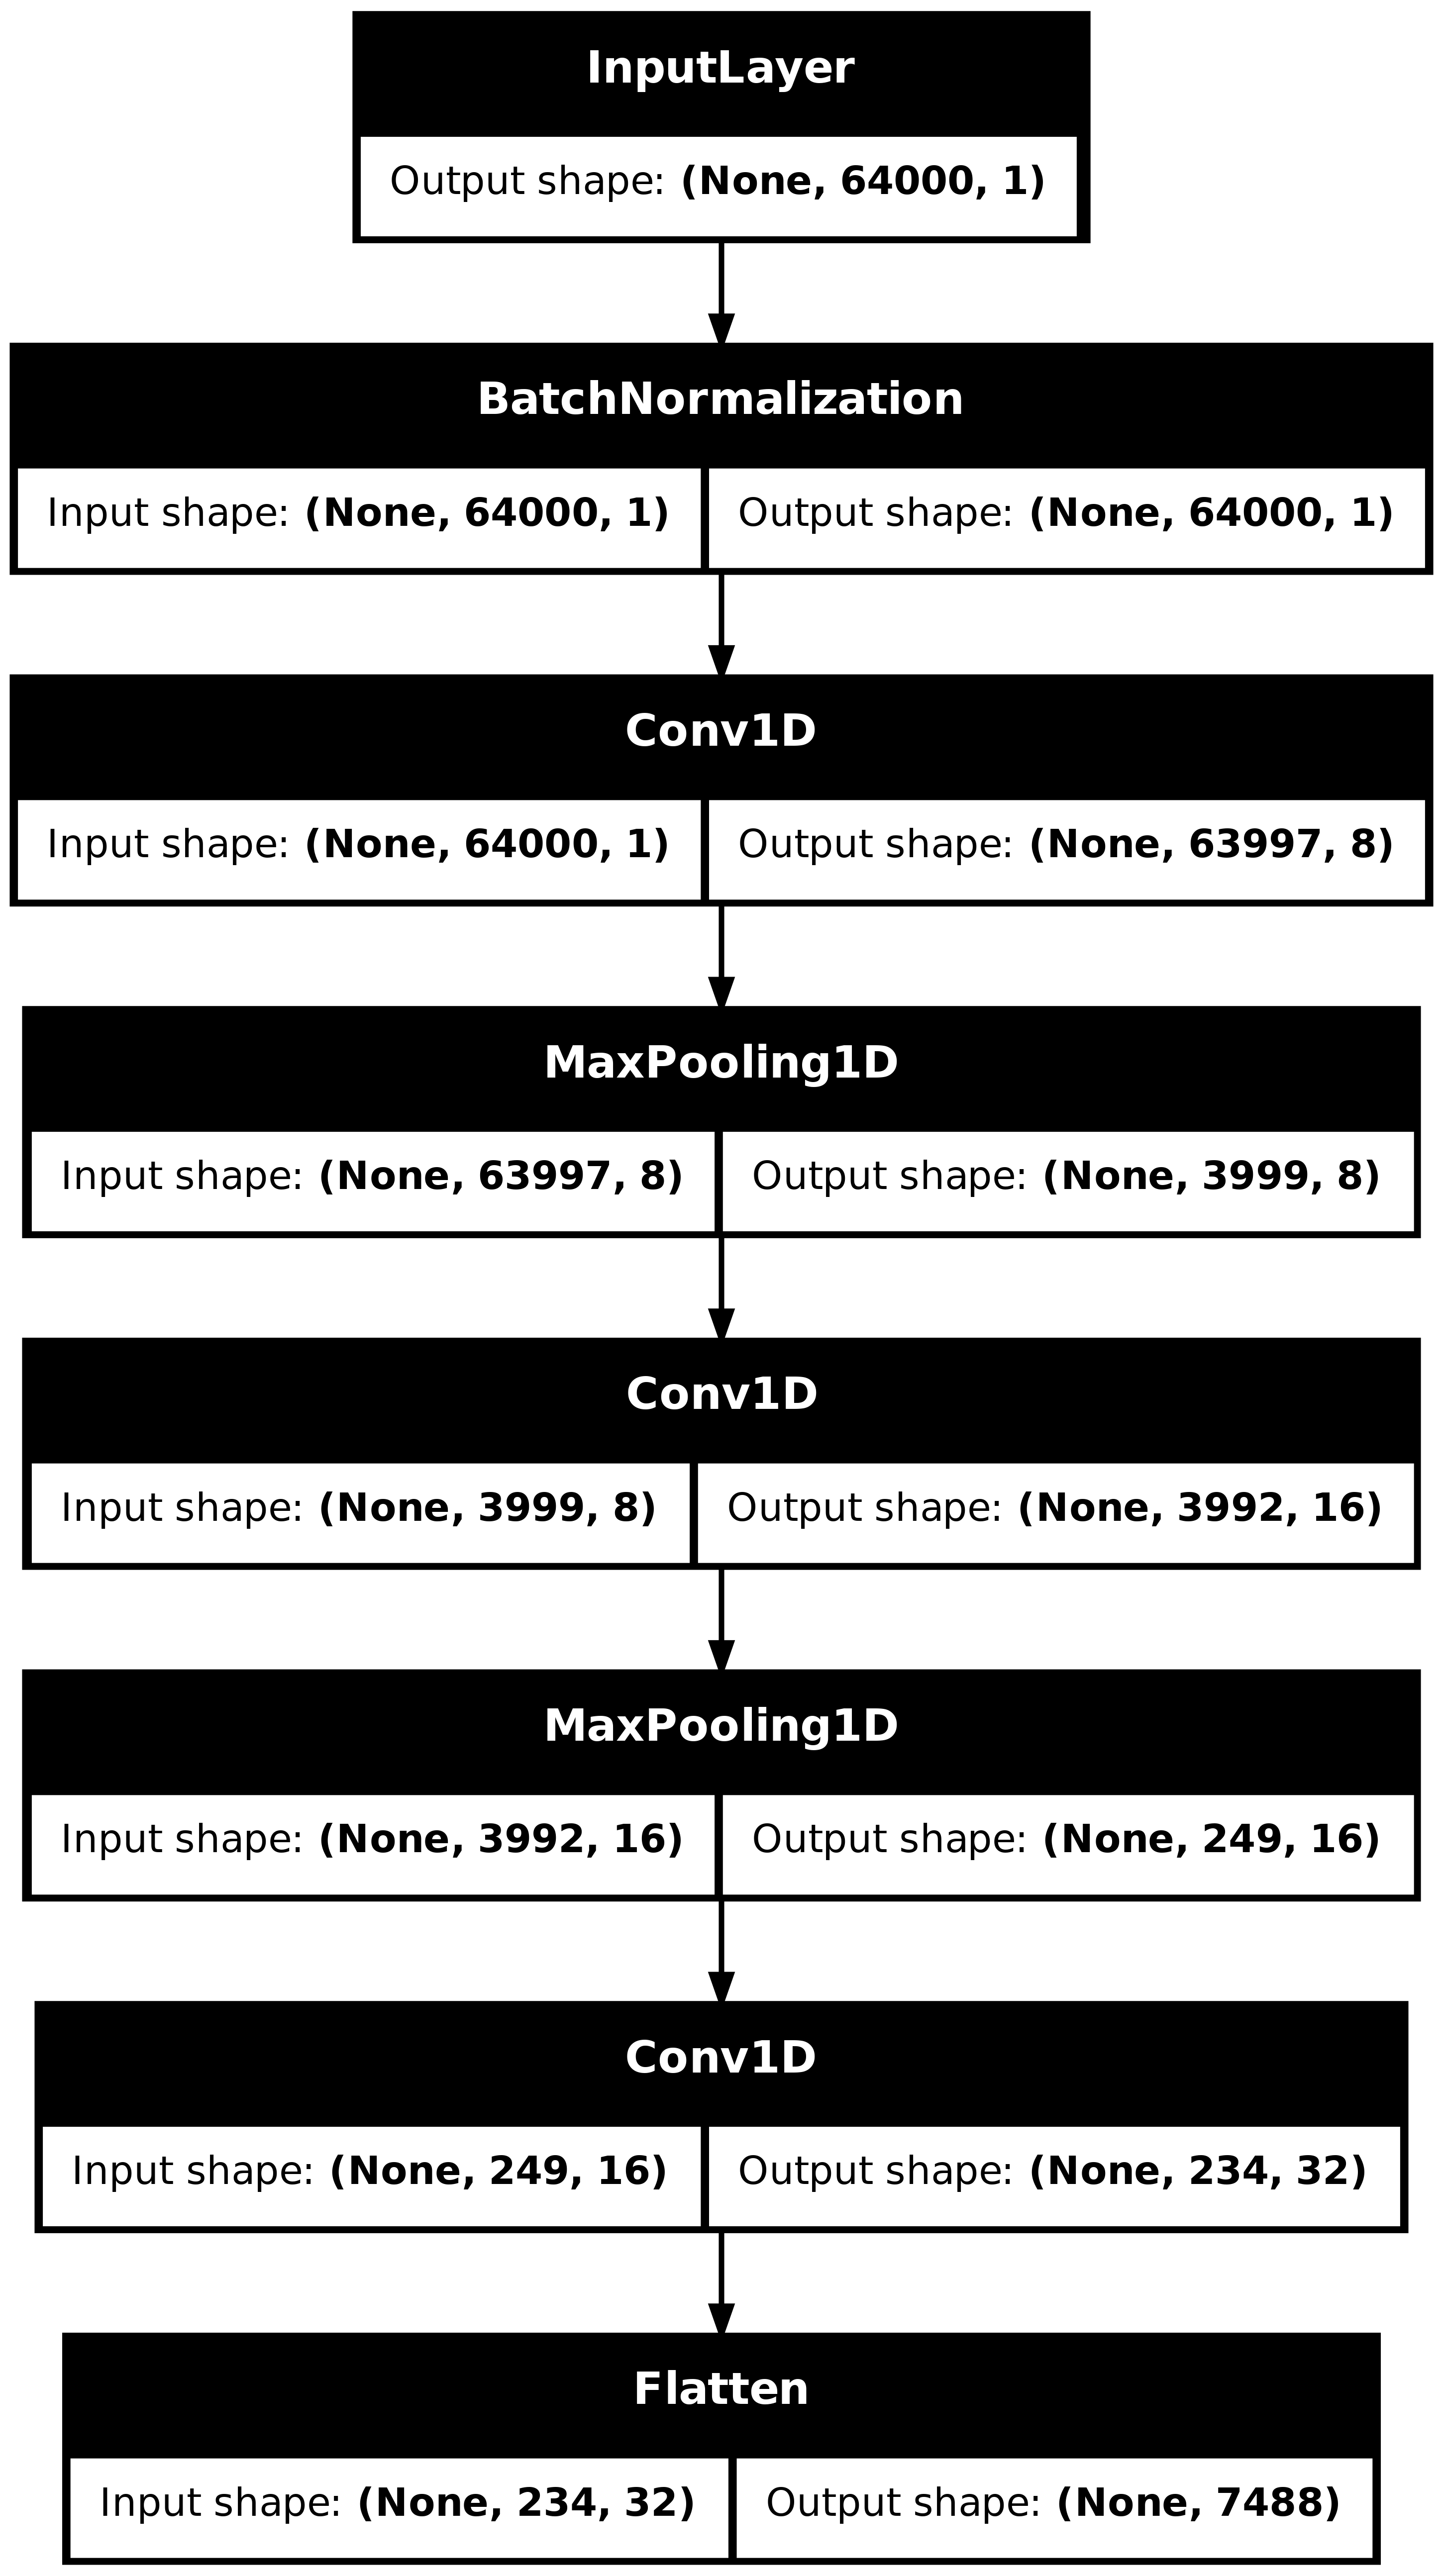
\includegraphics[width=0.21\textwidth,height=0.4\textwidth,trim={0 0 0 0.6cm},clip]{figs/rede1.png}} \label{fig:rede1}
    \qquad
    \subfloat[][Regressor]{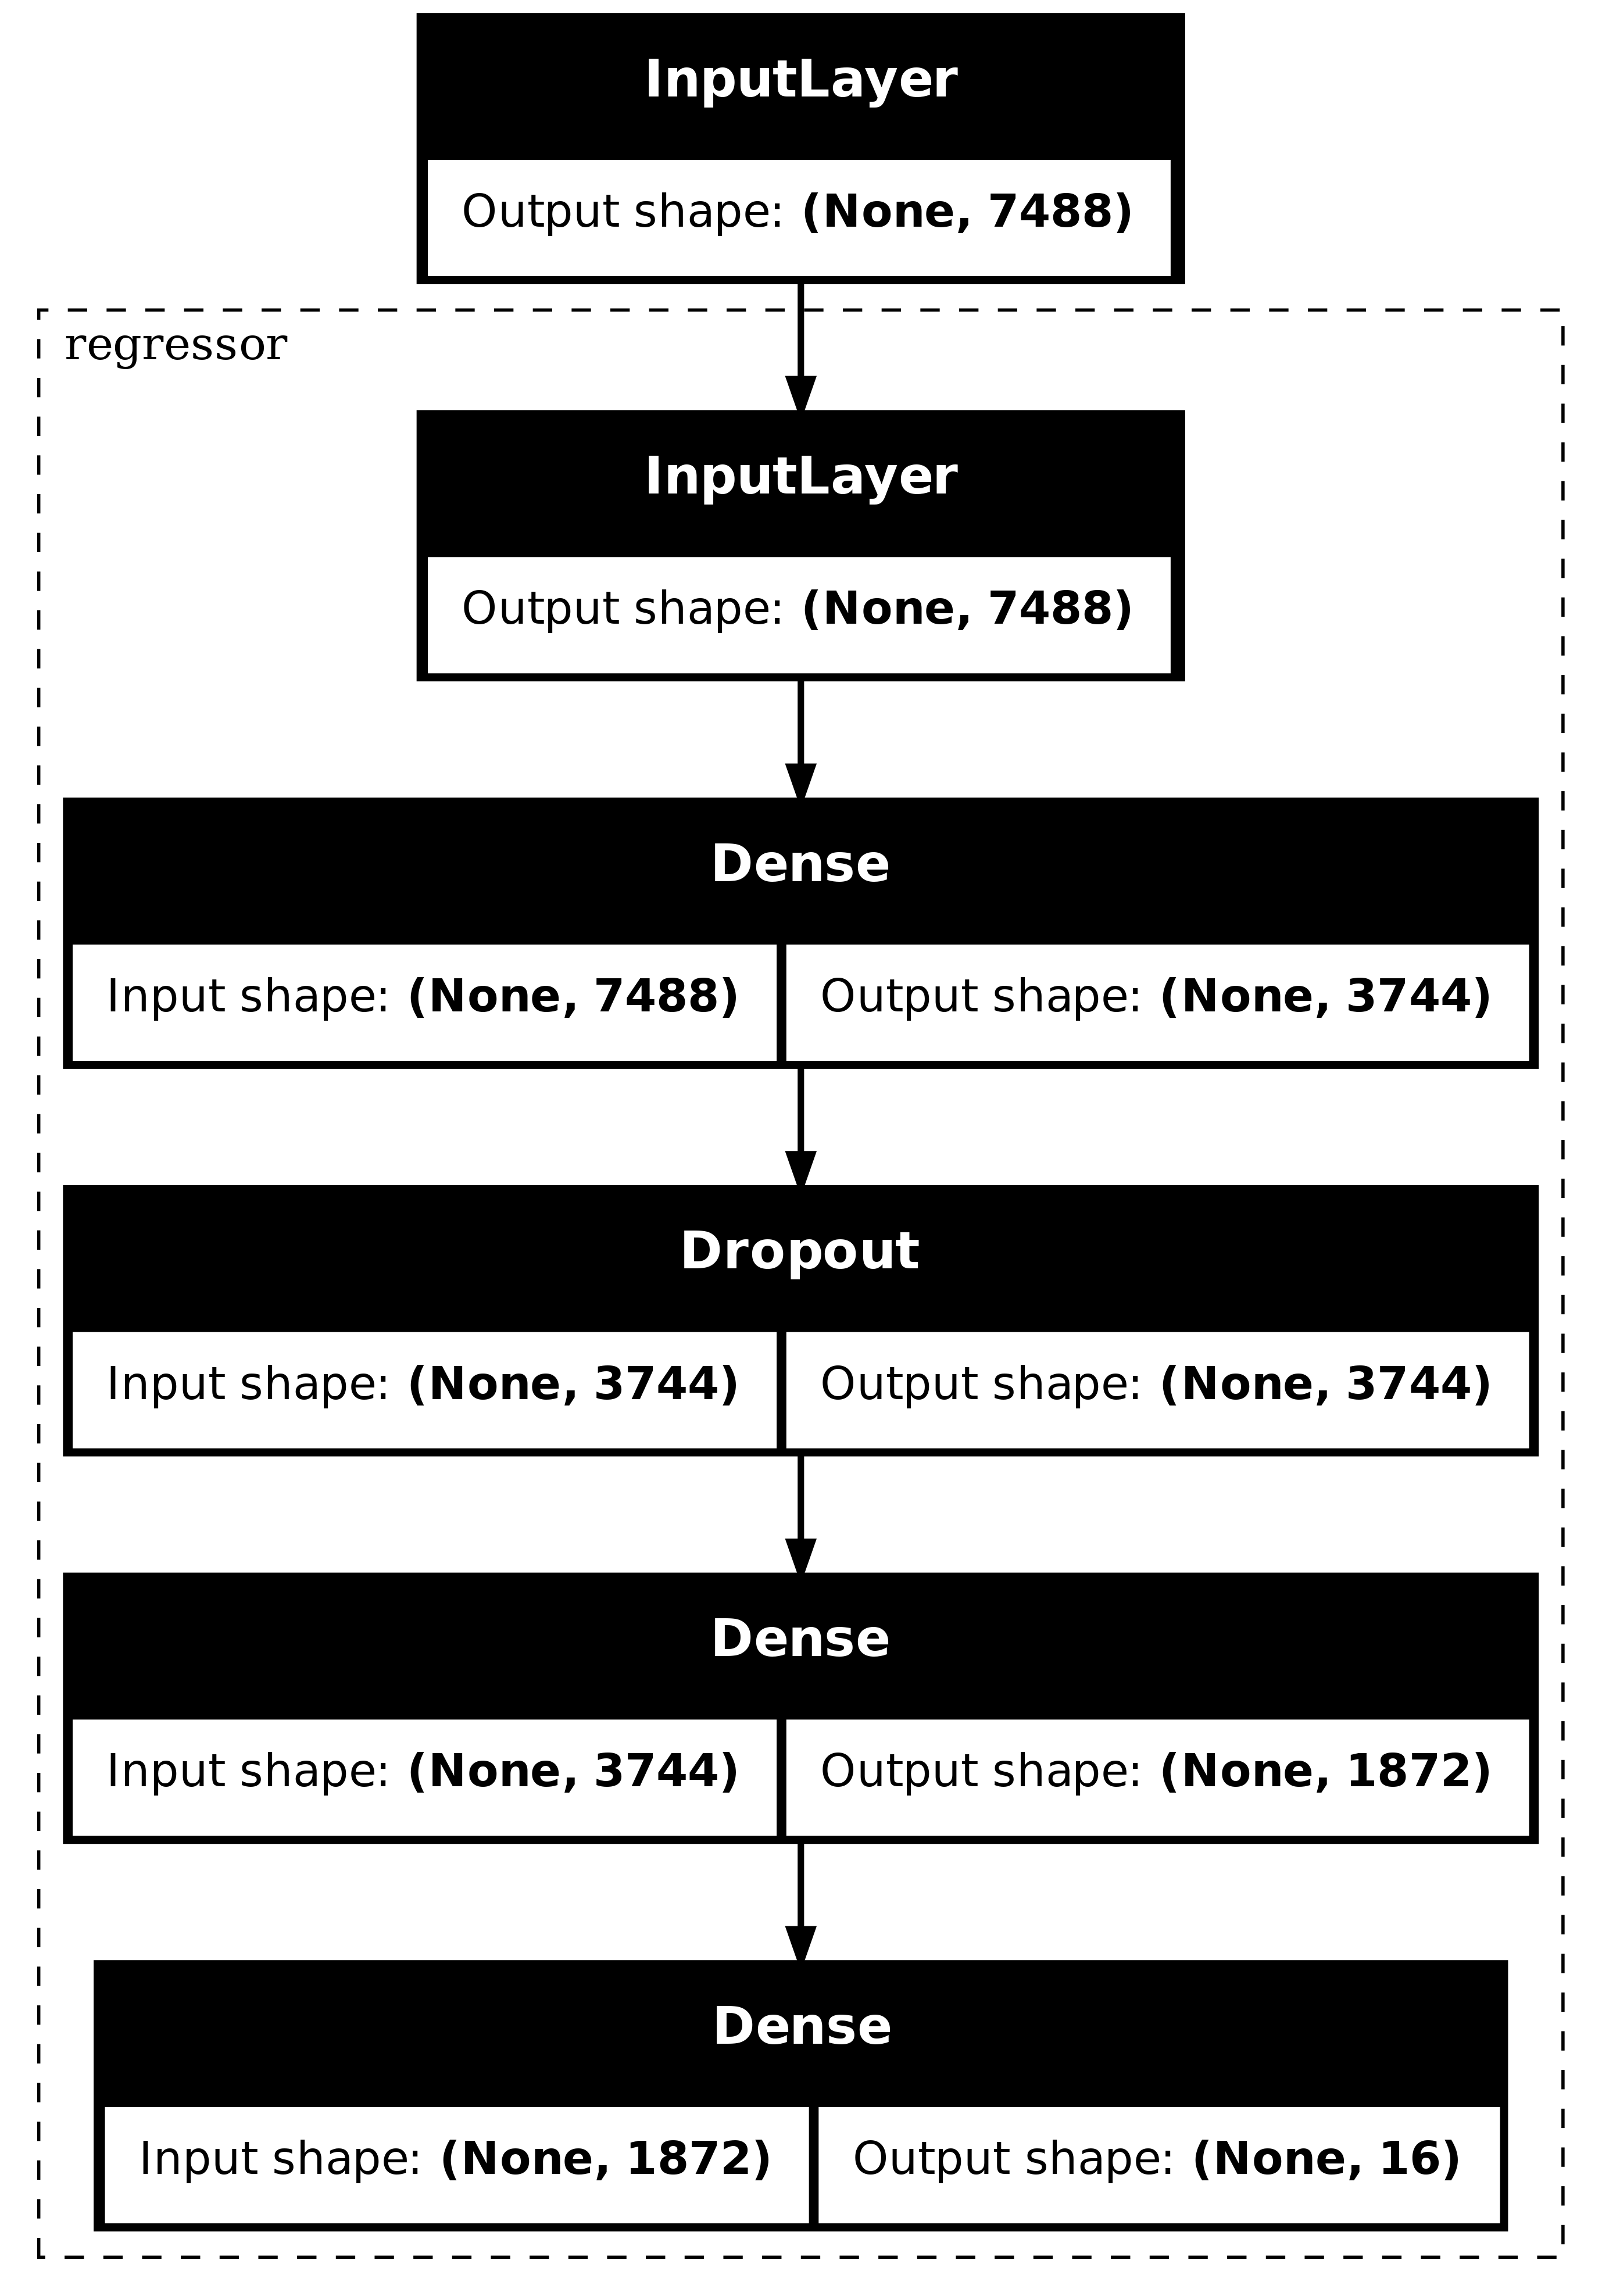
\includegraphics[width=0.21\textwidth,height=0.4\textwidth,trim={0 0 0 0.85cm},clip]{figs/rede2.png}} \label{fig:rede2}
    \caption{Overview of the entire Model Architecture}
    \label{fig:redes}
\end{figure}


The complete model is simply the sum of the two parts. But it is important to highlight the hyperparameters of each.

The feature-extraction part (CNN) comprises three sequential Conv1D–MaxPooling blocks. The first Conv1D layer uses 8 filters with a kernel size of 4 and stride 1, followed by a MaxPooling1D layer with pool size 16. The second Conv1D layer uses 16 filters with a kernel size of 8 and stride 1, followed by MaxPooling1D with pool size 16. The third Conv1D layer uses 32 filters with a kernel size of 16 and stride 1, followed by a final MaxPooling1D layer with pool size 16.

The regressor network part consists of two fully connected hidden layers followed by an output layer. The first dense layer uses the ReLU activation function and is followed by a dropout layer with a rate of 0.5 to mitigate overfitting. The second dense layer also employs the ReLU activation function. The output layer uses a linear activation (i.e., no activation function) to perform parameter regression. Model optimization is carried out using the Nadam optimizer.

Additional training settings include normalization of the target variables to zero mean and unit variance prior to training. The Nadam optimizer was employed, with mean squared error (MSE) used as the loss function, while mean absolute error (MAE) and MSE were recorded as evaluation metrics. The model was trained for up to 200 epochs using a batch size of 32, with early stopping enabled (patience of 20 epochs) and restoration of the best-performing weights.

\subsubsection{Hyperparameters Optimization}

To obtain the final architecture, a random search was performed over activation functions, regularization strategies, optimizers, and dropout rates. The best configuration was selected based on validation set performance. Although conceptually similar to a traditional grid search, this approach evaluates random combinations of hyperparameters, enabling broader coverage of the search space with reduced computational cost. The MLflow tool was used to track and compare training runs (additional details are available in the project repository).

The selected configuration employs the ReLU activation function, bias terms enabled in both the CNN and the regressor, a dropout rate of 0.5 in the regressor, no kernel regularization in the CNN, and L2 kernel regularization in the regressor.

\subsection{Evaluating the Model} \label{sec:evaluation_method}

After training the CNN, a new dataset is used to evaluate the model’s ability to re-synthesize real instruments by calculating specific metrics focused on the FM synthesizer’s capacity to reproduce the same timbres.

\begin{figure}[h]
    \centering
    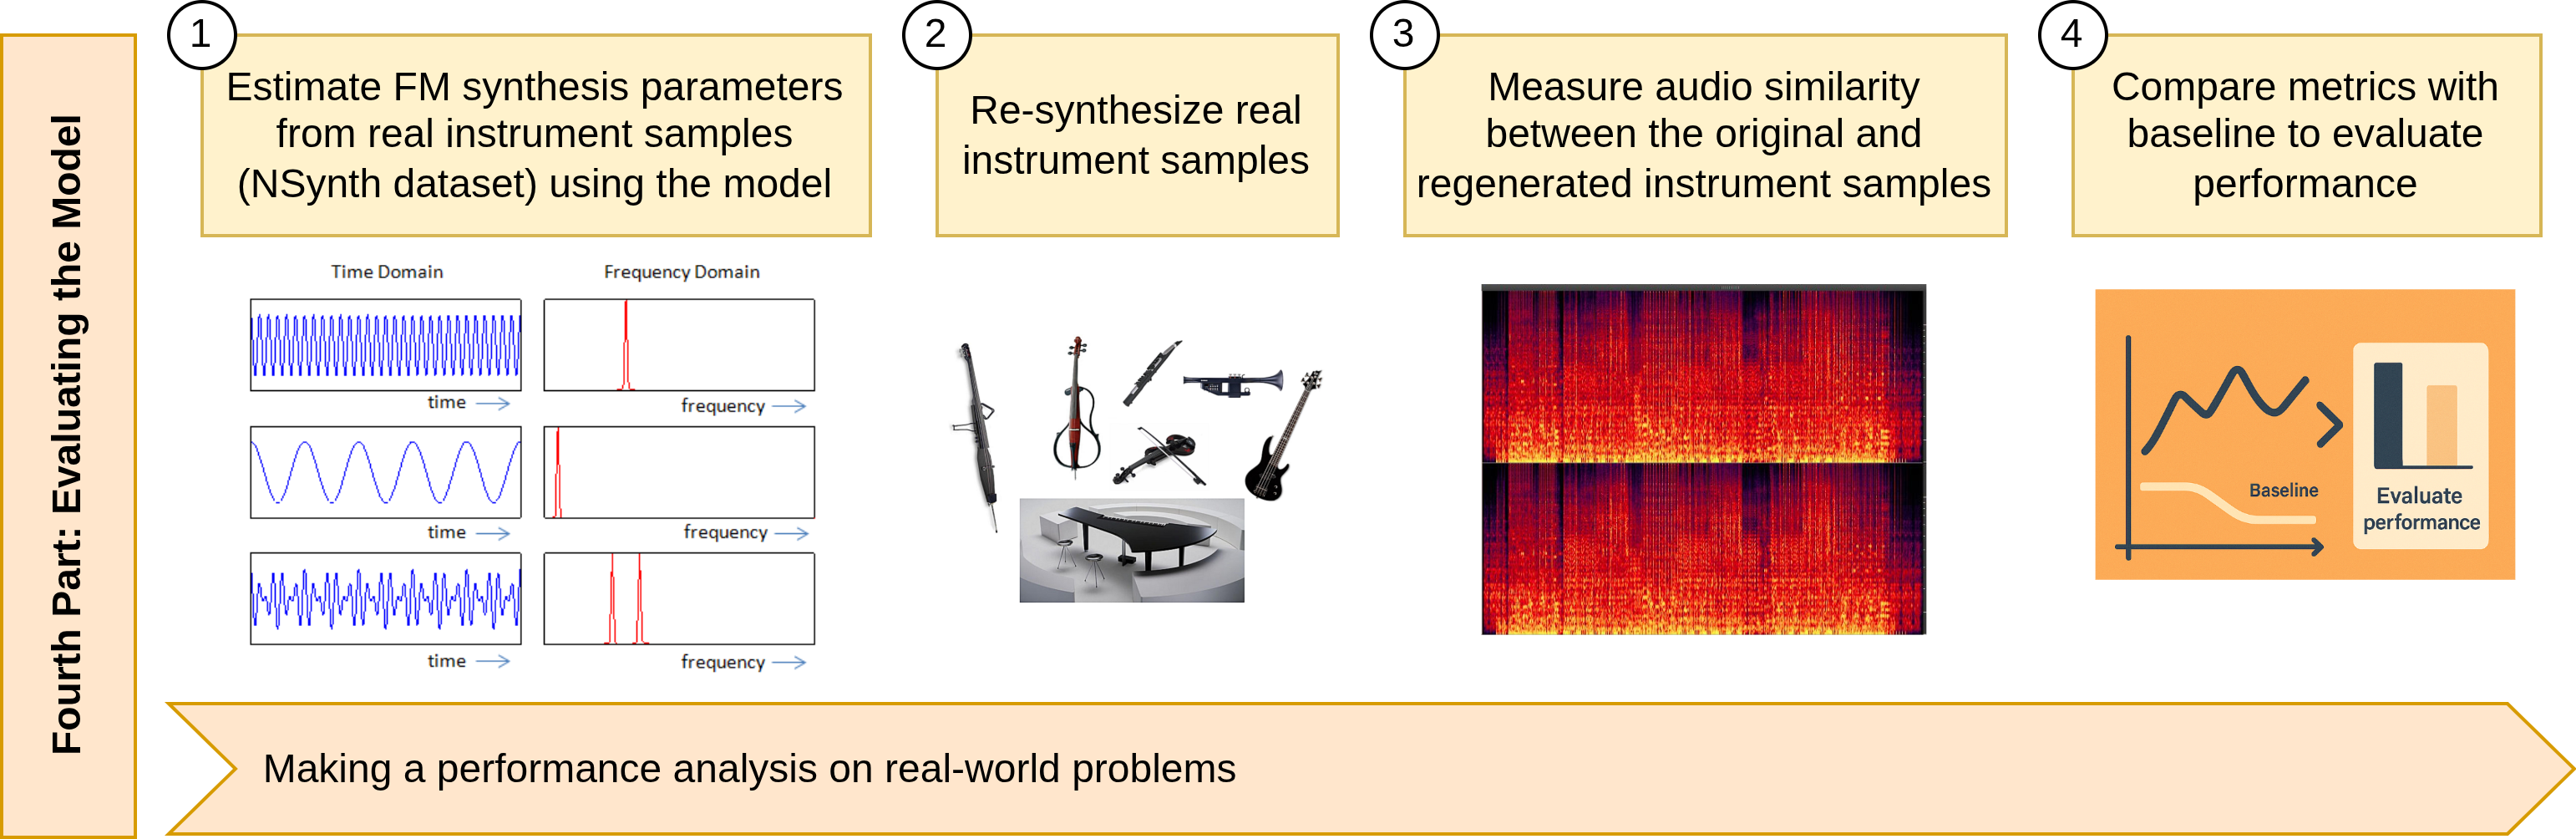
\includegraphics[width=1\columnwidth]{figs/fourth_part.png}
    \caption{Results evaluation.}
    \label{fig:met3}
\end{figure}

The NSynth dataset, part of Google’s Magenta project, contains numerous real instrument samples, including both acoustic and electronic instruments, as well as some synthetic sounds generated by professional synthesizers. This dataset has a configuration similar to that of the generated one used for training, and its main purpose is to evaluate the model’s generalization capabilities, since the model has never encountered it before.

Only the test split of the NSynth dataset was used in the evaluation, comprising 4,096 monophonic audio samples, each with a duration of 4 seconds and a sampling rate of 16~kHz. The dataset covers 11 instrument families, with pitches ranging from 27.5~Hz to 4,186.01~Hz, and employs amplitude envelopes consisting of up to 3 seconds of sustain followed by a 1-second decay.

The basic idea is to use the NSynth test samples as input to the model and, after predicting the synthesizer parameters, employ the implemented synthesizer to re-synthesize all samples. Finally, audio comparison metrics are calculated between each input and its corresponding generated sound, based on the proposed evaluation measures:

\begin{itemize}
    \item FFT distance: Used to compare the frequency components present in an audio signal.
    \item STFT distance: Used to compare the variation of frequency components over time.
    \item Log-mel-spectrogram distance: Used for a similar purpose as FFT distance, but typically models human cognitive pitch perception more accurately.
\end{itemize}

However, before using the predicted parameters as input to the synthesizer, a simple function was applied to approximate each ratio parameter to the nearest discrete ratio, according to the common behavior of musical harmonics (the same set of ratios used to randomize 90\% of the generated dataset). Furthermore, some clipping operations were also applied to enforce the same limits imposed on the randomly generated dataset, such as maximum and minimum values for beta parameters.

In order to achieve a good evaluation, the proposed metrics were also used to compare each NSynth audio with a baseline, which consists of a pure sinusoidal signal, with a frequency of 440 Hz (i.e., the A4 note, which is used as a reference to tune the majority of instruments).

\section{Experimental Results and Discussion}  \label{sec:experiments}

This section presents the final results of the model, considering both the training metrics and the audio comparision metrics. The former is used to evaluate the model’s ability to learn the entire parameter space, while the latter assesses its generalization capabilities, particularly its ability to emulate real instruments.

\subsection{Training Results}

The training and validation curves are shown in Figure~\ref{fig:mae_mse_evolution}. The model exhibits stable convergence, with no evidence of overfitting throughout the training process.

\begin{figure}[h]
 \centering
 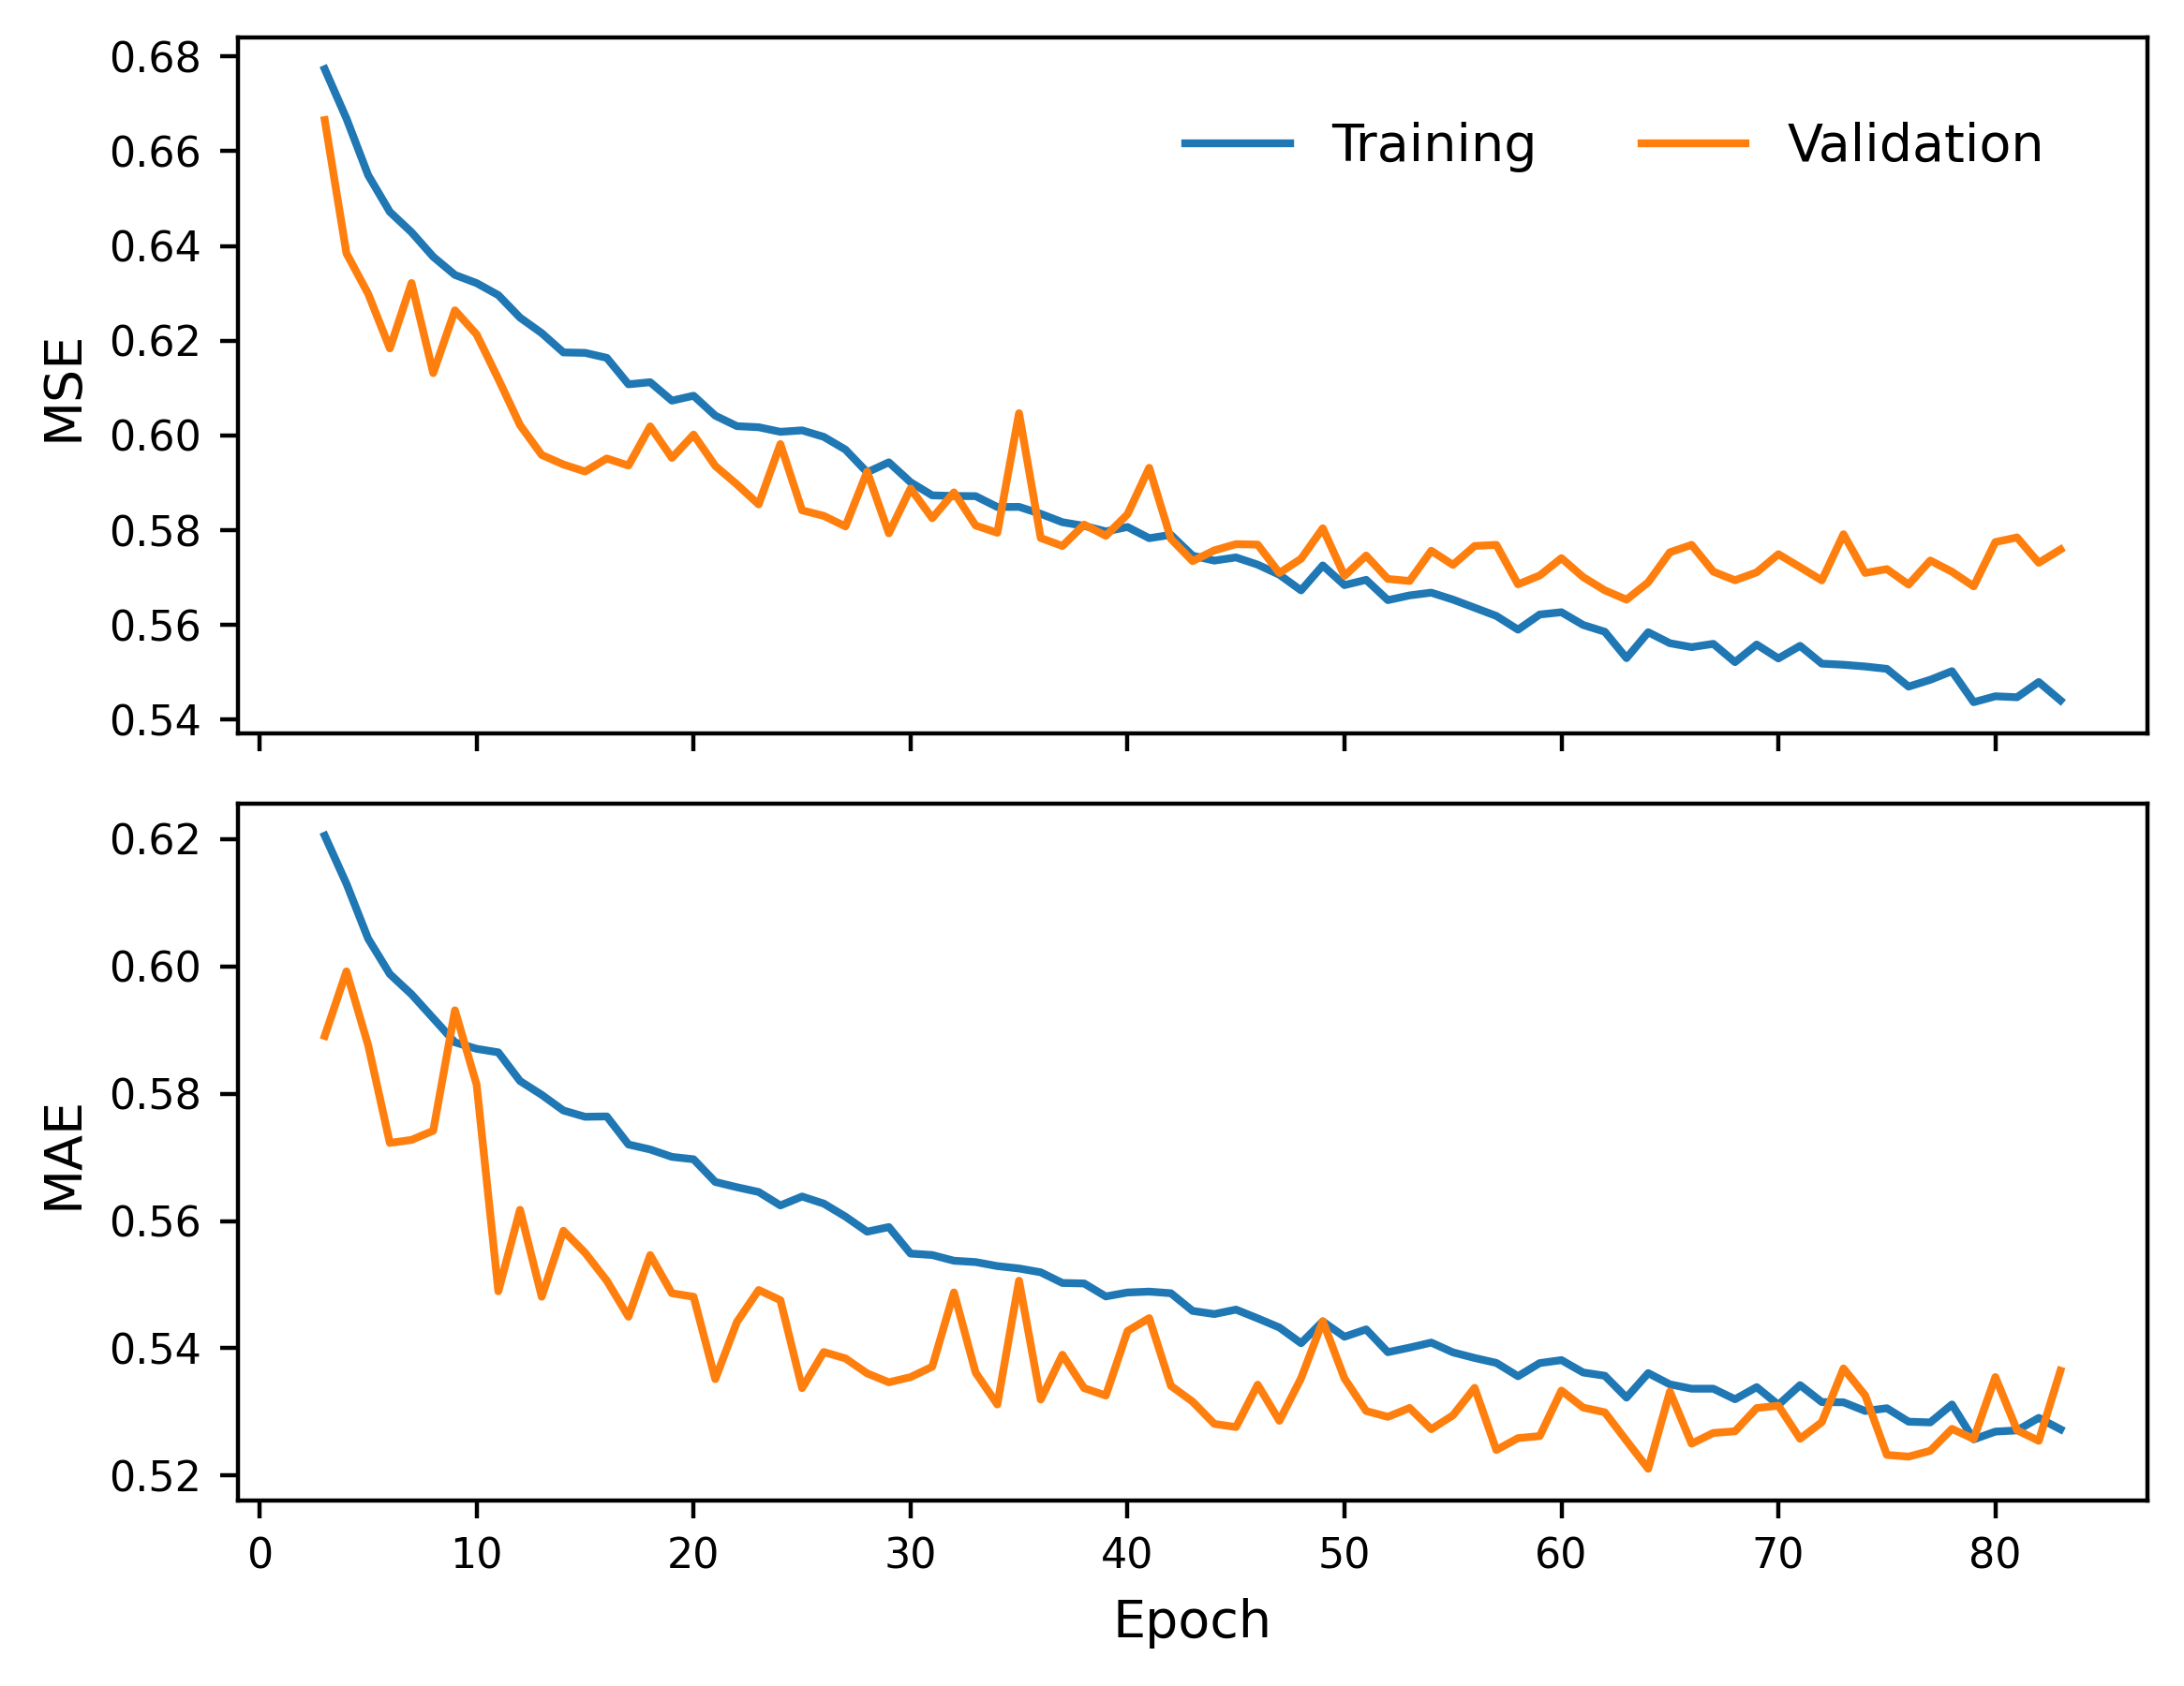
\includegraphics[width=\linewidth]{figs/mae_mse_evolution.png}
 \caption{Evolution of MAE and MSE during training.}
 \label{fig:mae_mse_evolution}
\end{figure}

After training, the model was evaluated on a held-out portion of the synthetic dataset. The predicted parameters were transformed back to their original scale, yielding a mean absolute error (MAE) of 6.488, a mean squared error (MSE) of 1410.097, and a root mean squared error (RMSE) of 37.551. These results indicate that the model is able to accurately reproduce the synthesizer parameters generated during the synthetic data creation process.


\subsection{Audio Comparision Results}

As presented in Section~\ref{sec:evaluation_method}, after training, the model’s generalization capabilities were tested through a process of re-synthesizing the NSynth dataset. The performance was evaluated by comparing the audio distance metrics between the original samples and the baseline samples with those between the re-synthesized samples and the original ones:


\begin{table}[htb] \small % desvios nas colunas
  \caption{Comparison between Resynthesis and Baseline with Improvement \% (considering mean and standard deviation).}
  \label{tab:metrics}
\begin{tabular*}{\columnwidth}
	{@{\extracolsep{\fill}}lcccc}
        \toprule
        & \multirow{2}{*}{FFT} & \multirow{2}{*}{STFT} & Log Mel & Log Mel \\ 
        & & & (raw) & (normalized) \\
        
        \midrule
        \multirow{2}{*}{Resynthesis} & 12649.9 & 2366.4 & 138.73 & 0.0086 \\
        & (6208.1) & (1132.2) & (47.013) & (0.0029) \\ 
        \multirow{2}{*}{Baseline} & 33508.8 & 7290.4 & 184.87 & 0.0115 \\
        & (1887.36) & (434.87) & (30.136) & (0.0019) \\
        \midrule
        Tuning (\%) & 62.270 & 67.540 & 24.960 & 24.930 \\
        \bottomrule
    \end{tabular*}
    \label{tab:metrics}
\end{table}


% \begin{table} \small % desvios nas colunas
%   \caption{Comparison between Resynthesis and Baseline with Improvement \% (considering mean and standard deviation).}
%   \label{tab:metrics}
% \begin{tabular*}{\columnwidth}
% 	{@{\extracolsep{\fill}}lccccc}
%     \toprule
%     Metric & Resynthesis & STD & Baseline & STD & Tuning (\%) \\
%     \midrule
%     FFT  & 12649.9 & 6208.1 & 33508.8 & 1887.36  & 62.270 \\
%     STFT  & 2366.4 & 1132.2  & 7290.4 & 434.87  & 67.540 \\
%     %Log Mel (raw)
%     Log Mel (r) & 138.73 & 47.013 & 184.87 & 30.136 & 24.960 \\
%     %Log Mel (normalized)
%     Log Mel (n) & 0.0086 & 0.0029  & 0.0115 & 0.0019 & 24.930 \\
%     \bottomrule
%   \end{tabular*}
%   \label{tab:metrics}
% \end{table}


Note that the Log Mel metric was compared, including a normalized version, which is obtained by dividing the raw Log Mel value by the product of the number of Mel bands and the time window quantity.

Furthermore, to facilitate a better understanding, the metrics were also compared by grouping the dataset by instrument family. This allows for the evaluation of the model's performance on different classes of sounds. Tables~\ref{tab:avg_metrics_groups} and \ref{tab:stdev_metrics_groups} show the average and standard deviation values, respectively. We can note that the top three best results were obtained for keyboard, guitar, and mallet families.


% \begin{table} \small
%   \caption{Comparison of Average by Instrument Group}
%   \label{tab:means_by_group_updated}
%   \begin{tabular}{lcccc}
%     \toprule
%     Group & FFT & STFT & Log Mel (raw) & Log Mel (norm) \\
%     \midrule
%     bass     & 11232.7 & 2144.32 & 135.610 & 0.00841 \\
%     brass    & 14371.1 & 2682.95 & 167.617 & 0.01039 \\
%     flute    & 14611.3 & 2872.69 & 141.819 & 0.00879 \\
%     guitar   & 9692.0  & 1867.47 & 119.853 & 0.00743 \\
%     keyboard & 9619.3  & 1772.92 & 119.529 & 0.00741 \\
%     mallet   & 8085.8  & 1632.45 & 120.610 & 0.00748 \\
%     organ    & 18360.1 & 3453.13 & 166.433 & 0.01032 \\
%     reed     & 12740.0 & 2267.08 & 140.701 & 0.00872 \\
%     string   & 12883.7 & 2390.65 & 139.365 & 0.00864 \\
%     vocal    & 31028.9 & 5271.26 & 212.646 & 0.01319 \\
%     \bottomrule
%   \end{tabular}
%   \label{tab:avg_metrics_groups}
% \end{table}

\begin{table}[htb] \small
  \caption{Average values by Instrument Group.}
  \label{tab:means_by_group_updated}
  \begin{tabular*}{\columnwidth}
	{@{\extracolsep{\fill}}lcccc}
  %\begin{tabular}{lcccc}
    \toprule
    \multirow{2}{*}{Group} & \multirow{2}{*}{FFT} & \multirow{2}{*}{STFT} & Log Mel& Log Mel \\
    &   &   &   (raw)  & (normalized) \\
    \midrule
    bass     & 11232.7 & 2144.32 & 135.610 & 0.00841 \\
    brass    & 14371.1 & 2682.95 & 167.617 & 0.01039 \\
    flute    & 14611.3 & 2872.69 & 141.819 & 0.00879 \\
    guitar   & 9692.0  & 1867.47 & 119.853 & 0.00743 \\
    keyboard & 9619.3  & 1772.92 & 119.529 & 0.00741 \\
    mallet   & 8085.8  & 1632.45 & 120.610 & 0.00748 \\
    organ    & 18360.1 & 3453.13 & 166.433 & 0.01032 \\
    reed     & 12740.0 & 2267.08 & 140.701 & 0.00872 \\
    string   & 12883.7 & 2390.65 & 139.365 & 0.00864 \\
    vocal    & 31028.9 & 5271.26 & 212.646 & 0.01319 \\
    \bottomrule
  \end{tabular*}
  \label{tab:avg_metrics_groups}
\end{table}


\section{Conclusion} \label{sec:conclusion}

This work aimed to develop and evaluate a technique capable of achieving two primary objectives: re-synthesizing the sounds of real musical instruments and exploring the synthesizer’s parameter space in a randomized manner to assess the model’s generalization capacity. The proposed convolutional neural network (CNN) model demonstrated strong performance in both aspects, effectively reproducing real instrument timbres and showing satisfactory generalization when exposed to unseen parameter configurations. The re-synthesized audios, when compared to the original samples from the NSynth dataset, confirmed the model’s ability to approximate realistic timbral characteristics, while maintaining consistent performance across different instrument families. The stability of the normalized log-mel metric across all categories suggests that the model is not overly biased toward specific timbral structures, reinforcing its robustness and flexibility. These results validate the initial hypothesis that CNNs are highly efficient in extracting relevant spectral and temporal features from audio signals, and that randomized dataset generation can effectively guide the learning process, enabling a level of control over FM synthesis parameters sufficient to emulate real-world sounds.

Despite these promising outcomes, the approach presents some limitations that delineate directions for future research. First, the use of a dataset restricted to musical instruments limits the generalization potential of the system; therefore, future experiments should incorporate more diverse sound sources, such as environmental or synthetic noises, to enhance creative applicability. Additionally, the adoption of a single linear ADSR envelope constrained the diversity of synthesized dynamics, indicating that broader variations should be implemented to better model non-instrumental or abstract sound categories. Another limitation concerns the exploration of FM synthesis algorithms, as only two were tested, and a single configuration yielded satisfactory results; expanding this investigation to include more complex operator topologies could significantly improve the synthesis flexibility.

Future work should thus focus on testing alternative neural architectures, such as autoencoders, to improve feature representation and generalization, as well as combining CNN-based feature extraction with other strategies found in the literature, including the use of STFT-based regression inputs or perceptually informed loss functions such as the log-mel metric. Moreover, the application of AutoML techniques could optimize the regression stage of the pipeline, potentially enhancing the model’s predictive performance. Finally, retraining the model using a professional FM synthesizer implementation would provide a more realistic framework for evaluation and deployment, advancing the state of neural sound synthesis and broadening its relevance for both academic research and creative audio production.

\section*{Acknowledgment}

Omitted due to blind review.

\balance

% \begin{acks}
% This work is supported by \textit{Coordenação de Aperfeiçoamento de Pessoal de Nível Superior}~(CAPES), \textit{Conselho Nacional de Desenvolvimento Científico e Tecnológico}~(CNPq), grants 406417/2022-9, 102475/2024-5, and 312209/2022-3, and \textit{Fundação de Amparo à Pesquisa do Estado de São Paulo}~(FAPESP), grant 2020/09835-1~(CPA IARA). 
% \end{acks}


%%
%% Print the bibliography
%%

\bibliographystyle{IEEEtran}
\bibliography{bib/references, bib/sample-base, bib/software}

\end{document}
